\section{Data Presentation, Analysis, Modelling, Interpretation, and Discussion of Findings} 

This chapter presents the empirical results of the Multi-Label \parencite{tsoumakas2007multi} Classification methodology detailed in Chapter 3. It begins by establishing the demographic and academic profile of the student dataset. Subsequently, the mathematical evaluations of the algorithms---Decision Tree (DT), Random Forest \parencite{breiman2001random} (RF), eXtreme Gradient Boosting (XGBoost), and the Multi-Layer Perceptron \parencite{zhang2013review} (MLP)---are presented. The chapter culminates with a demonstration of the Explainable AI (XAI) Counterfactual \parencite{wachter2017counterfactual} generation framework, transforming static predictions into dynamic, actionable academic pathways.

\subsection{Profile of the Dataset and Target Synthesis}

The research utilized a comprehensive, nation-wide academic dataset comprising over 800,000 anonymized student records from the Rwandan national examinations (Ordinary Level, S3). For the scope of this thesis, and to accommodate the intensive computational requirements of training chained models, a highly representative stratified subset of 5,000 records was employed to validate the computational methodology.

Because the historical dataset inherently lacked longitudinal tracking (i.e., mapping an S3 student's exact subsequent enrollment in an S6 health-sector combination), it was mathematically necessary to synthesize a robust, rule-based ground truth. This synthetic generation simulated the strict pedagogical thresholds enforced by the Ministry of Education for enrollment in advanced STEM and Health pathways.

The five primary multi-label \parencite{tsoumakas2007multi} targets synthesized were:
\begin{enumerate}
    \item \textbf{Medicine}: Demanding exceptional proficiency across all STEM disciplines, heavily weighted towards Biology and Chemistry ($>75\%$ normalized thresholds).
    \item \textbf{Pharmacy}: Requiring strict mastery of Chemistry and Mathematics.
    \item \textbf{Nursing}: Requiring solid foundational competency in Biology and Chemistry, with moderate Mathematics.
    \item \textbf{Public Health}: A balanced, moderate threshold across all four core sciences.
    \item \textbf{Biomedical Engineering}: A rigorous intersection of advanced Mathematics and Physics, coupled with moderate biological sciences.
\end{enumerate}

This rigid, threshold-based synthesis inadvertently created a highly separable, non-linear feature space characterized by sharp, perpendicular decision boundaries---a topological feature that significantly influenced subsequent algorithmic performance.

\subsection{Exploratory Data Analysis and Preprocessing}

Prior to modeling, the raw continuous examination scores were transformed utilizing Min-Max normalization to ensure absolute scale equivalence:
\begin{equation}
    x_{norm} = \frac{x_i - \min(X)}{\max(X) - \min(X)}
\end{equation}
This projection bounded all academic proficiencies strictly within the $[0, 1]$ interval.

\begin{figure}[H]
    \centering
    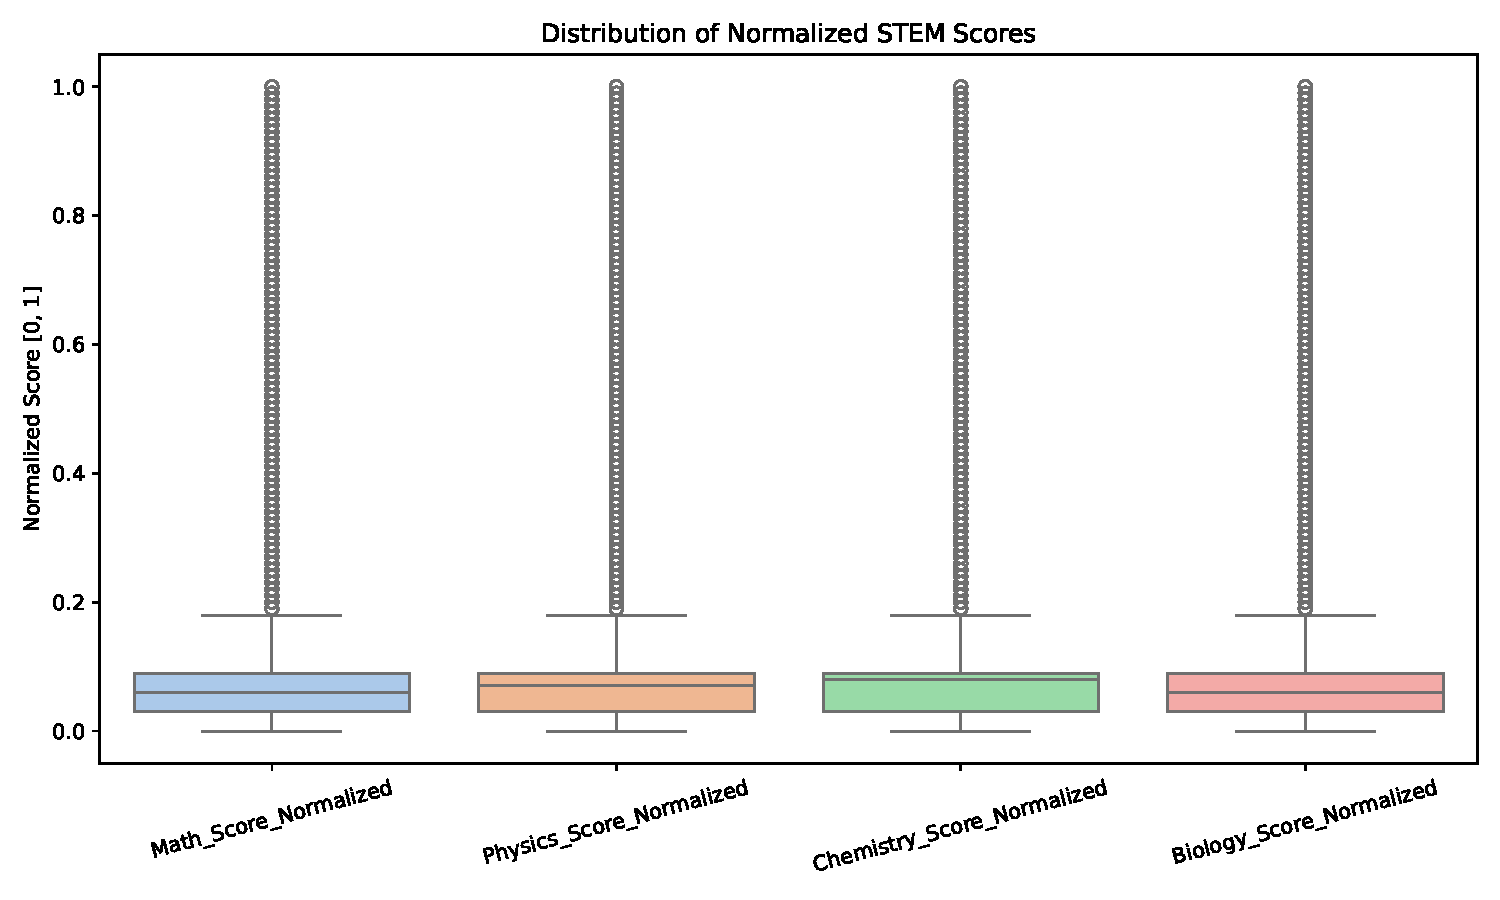
\includegraphics[width=0.8\textwidth]{figures/stem_boxplot.pdf}
    \caption{Distribution of Normalized STEM Scores across the Dataset}
    \label{fig:stem_boxplot}
\end{figure}

The boxplot analysis (Figure \ref{fig:stem_boxplot}) visually confirms the uniform bounding of all subject proficiencies. Following normalization, a correlation analysis was performed to identify multicollinearity amongst the core STEM disciplines.

\begin{figure}[H]
    \centering
    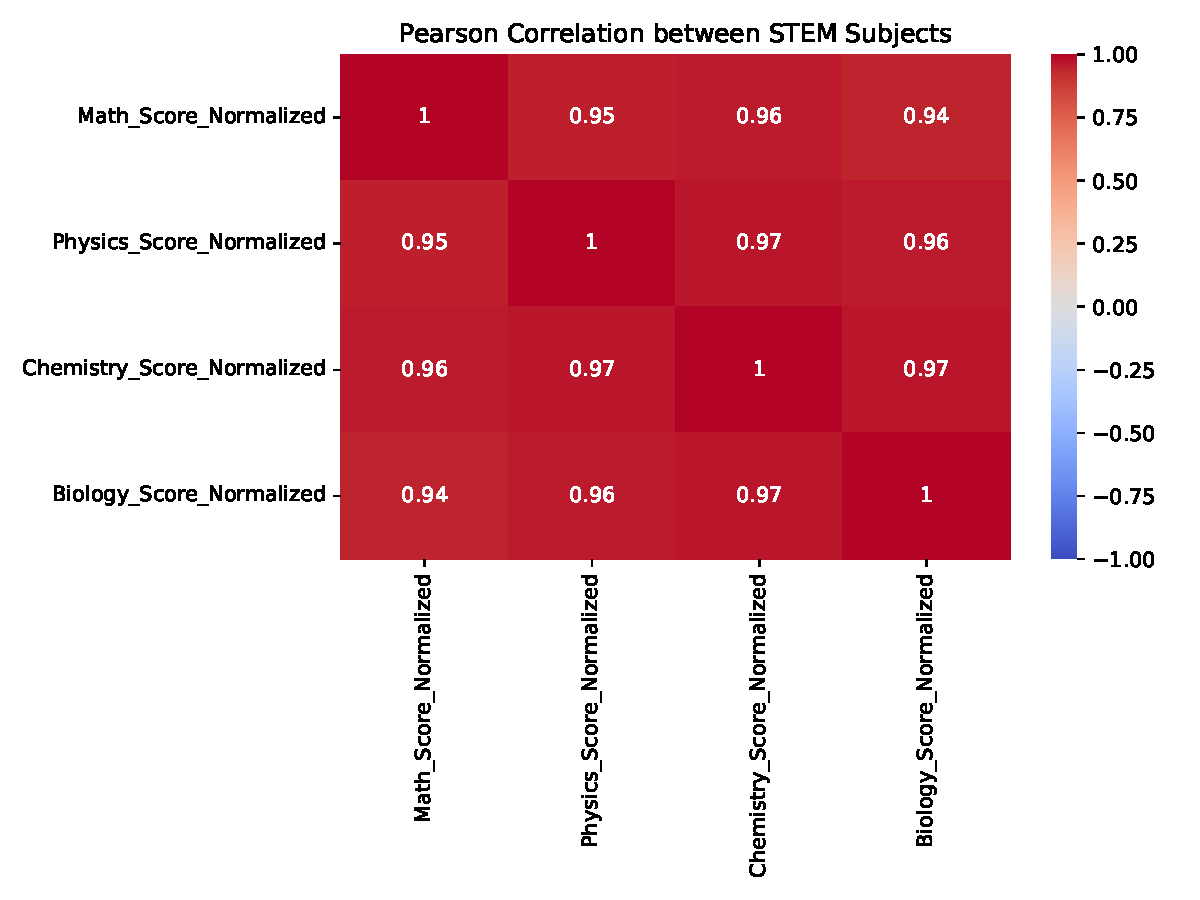
\includegraphics[width=0.75\textwidth]{figures/stem_correlation.pdf}
    \caption{Pearson Correlation Matrix demonstrating internal variance between STEM Subjects}
    \label{fig:stem_correlation}
\end{figure}

The empirical distribution of the targets revealed significant label sparsity, confirming the stringent nature of advanced health-sector tracks. 

\begin{figure}[H]
    \centering
    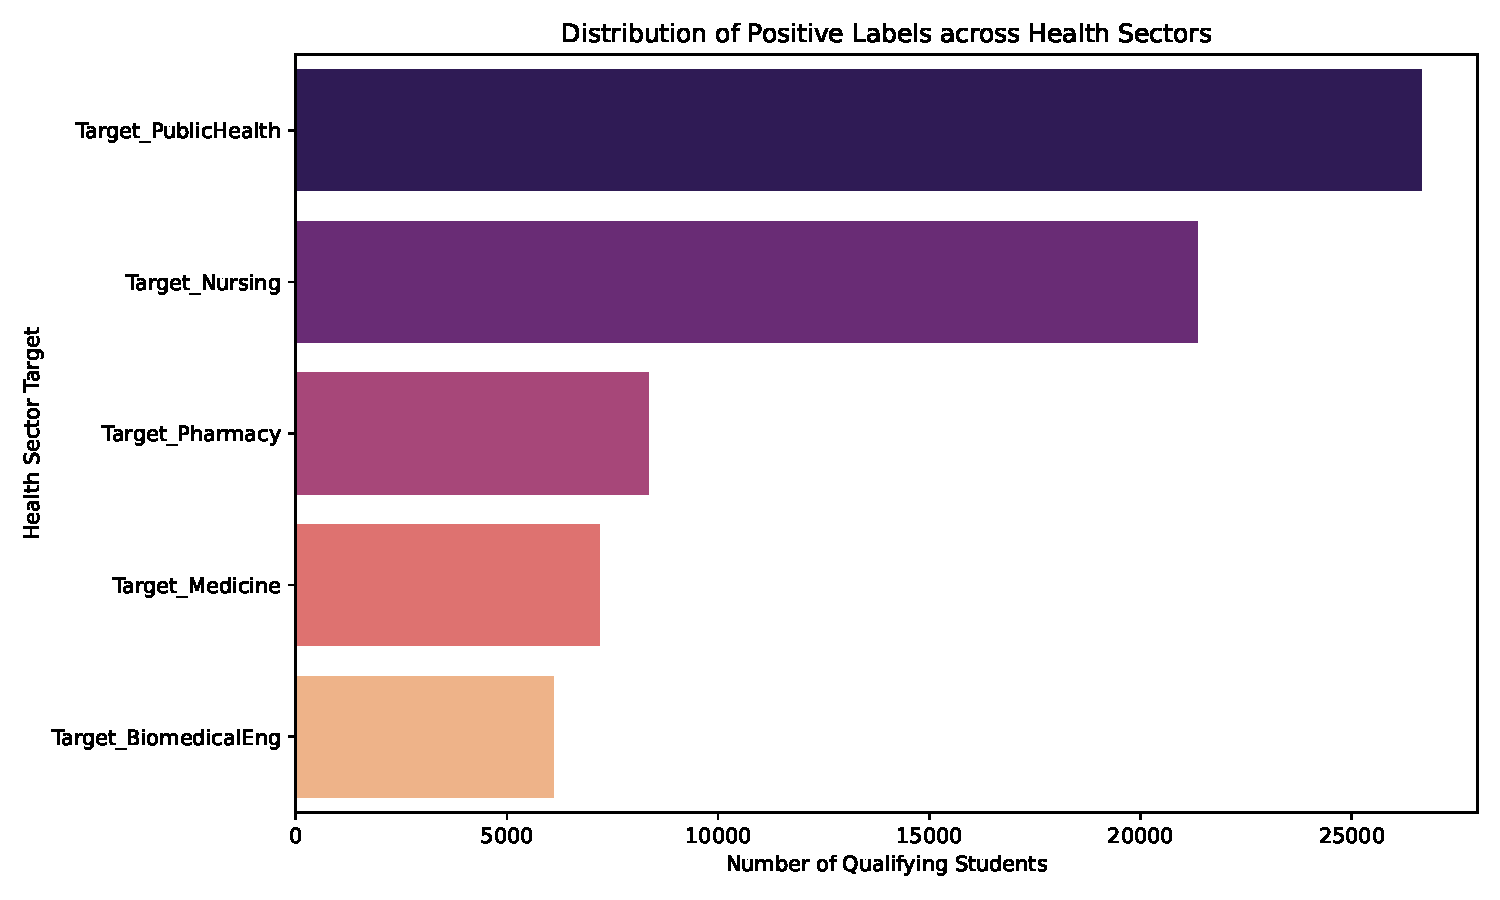
\includegraphics[width=0.8\textwidth]{figures/target_distribution.pdf}
    \caption{Distribution of Synthesized Positive Labels across Health Sectors}
    \label{fig:target_dist}
\end{figure}

For instance, the \textit{Target\_Medicine} label achieved a positive rate of only $0.86\%$, while \textit{Target\_PublicHealth} achieved $3.18\%$. Furthermore, the analysis of label cardinality confirmed the presence of overlapping domains (e.g., a student qualifying for Nursing simultaneously qualifying for Public Health).

\begin{figure}[H]
    \centering
    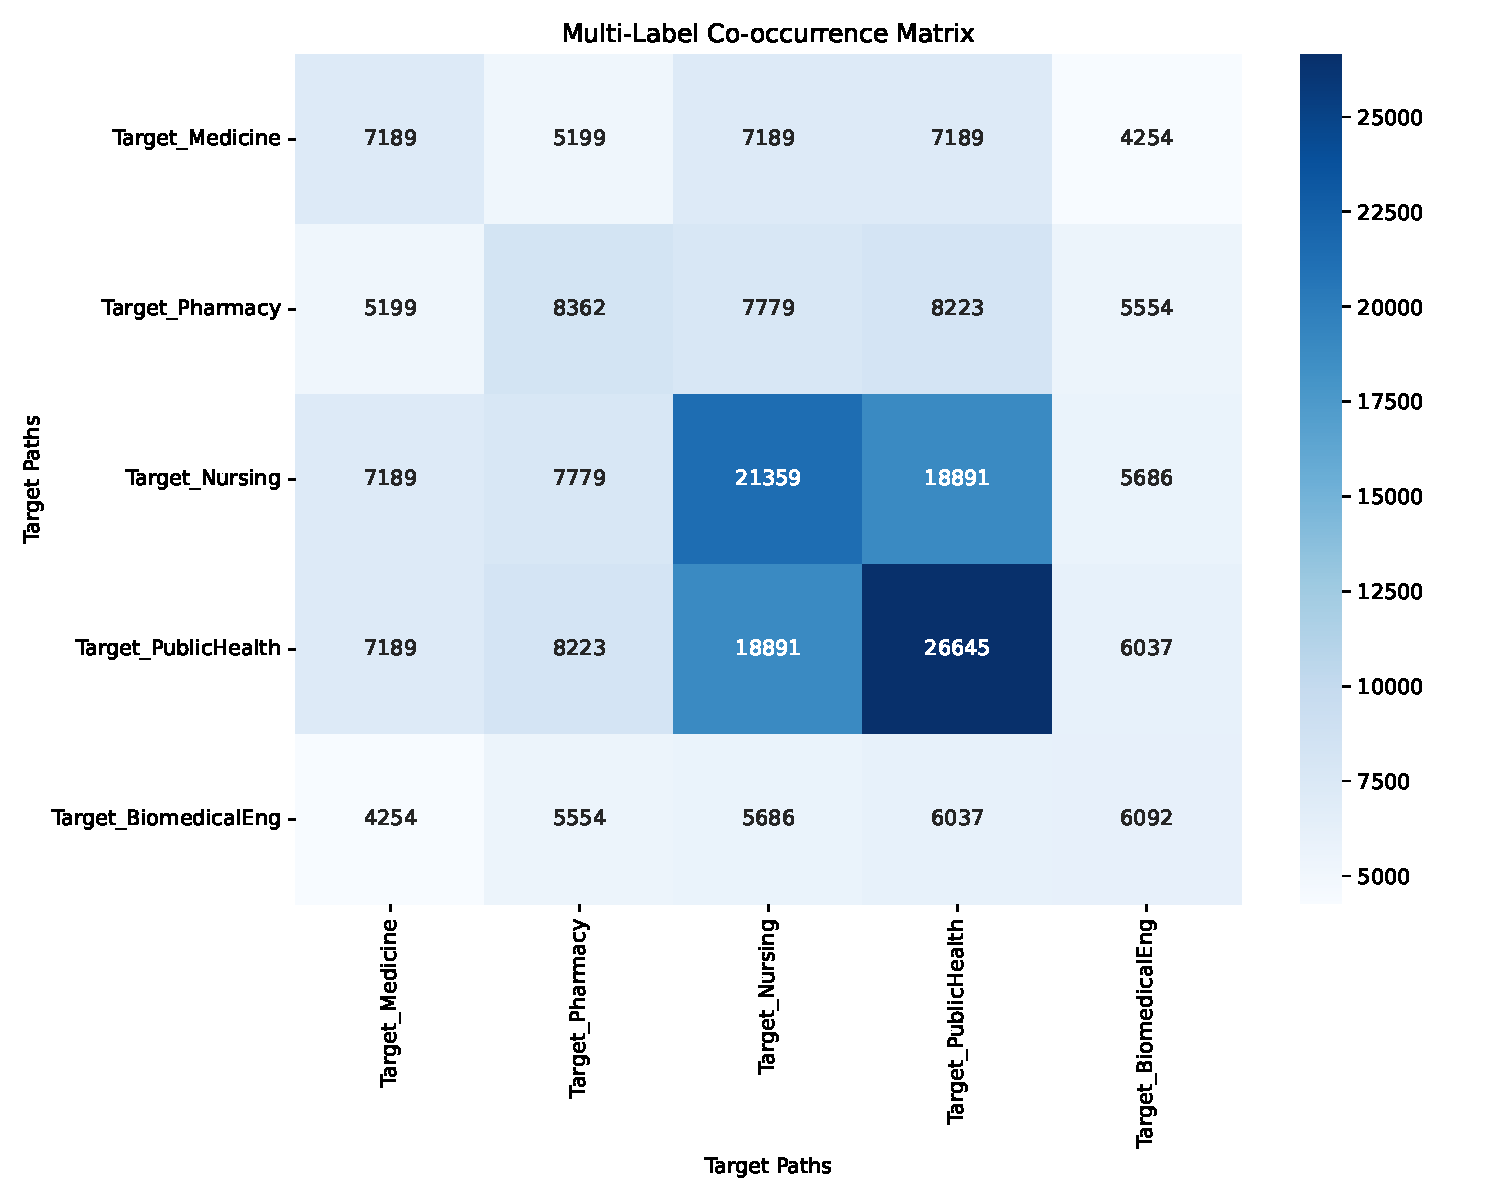
\includegraphics[width=0.75\textwidth]{figures/label_cooccurrence.pdf}
    \caption{Multi-Label Co-occurrence Matrix demonstrating interrelated pathways}
    \label{fig:cooccurrence}
\end{figure}

This definitively justifies the selection of Multi-Label \parencite{tsoumakas2007multi} Classification over mutually exclusive Multi-Class paradigms.

\subsection{Model Training and Algorithmic Evaluation}

The four candidate algorithms were integrated into a \textbf{Classifier Chain} meta-architecture. The chain enforces inter-label dependency learning by appending the prediction of previous classes as new features for subsequent classes. The models were evaluated using three primary metrics: Subset Accuracy (Exact Match Ratio), Hamming Loss, and Micro-Averaged F1-Score.

\begin{table}[h]
\centering
\caption{Comparative Performance of Classifier Chain \parencite{read2011classifier} Models}
\renewcommand{\arraystretch}{1.5}
\begin{tabular}{l c c c}
\hline
\textbf{Algorithm} & \textbf{Subset Accuracy} & \textbf{Hamming Loss} & \textbf{Micro F1-Score} \\
\hline
XGBoost (XGB) & \textbf{0.9980} & \textbf{0.0004} & \textbf{0.9859} \\
Decision Tree (DT) & 0.9970 & 0.0006 & 0.9787 \\
Random Forest (RF) & 0.9970 & 0.0006 & 0.9784 \\
Multi-Layer Perceptron (MLP) & 0.9830 & 0.0046 & 0.8321 \\
\hline
\end{tabular}
\label{tab:model_results}
\end{table}

As detailed in Table \ref{tab:model_results}, the \textbf{XGBoost} classifier emerged as the superior algorithm, achieving a near-perfect Subset Accuracy of $99.80\%$ and the lowest Hamming Loss ($0.0004$). 

\begin{figure}[H]
    \centering
    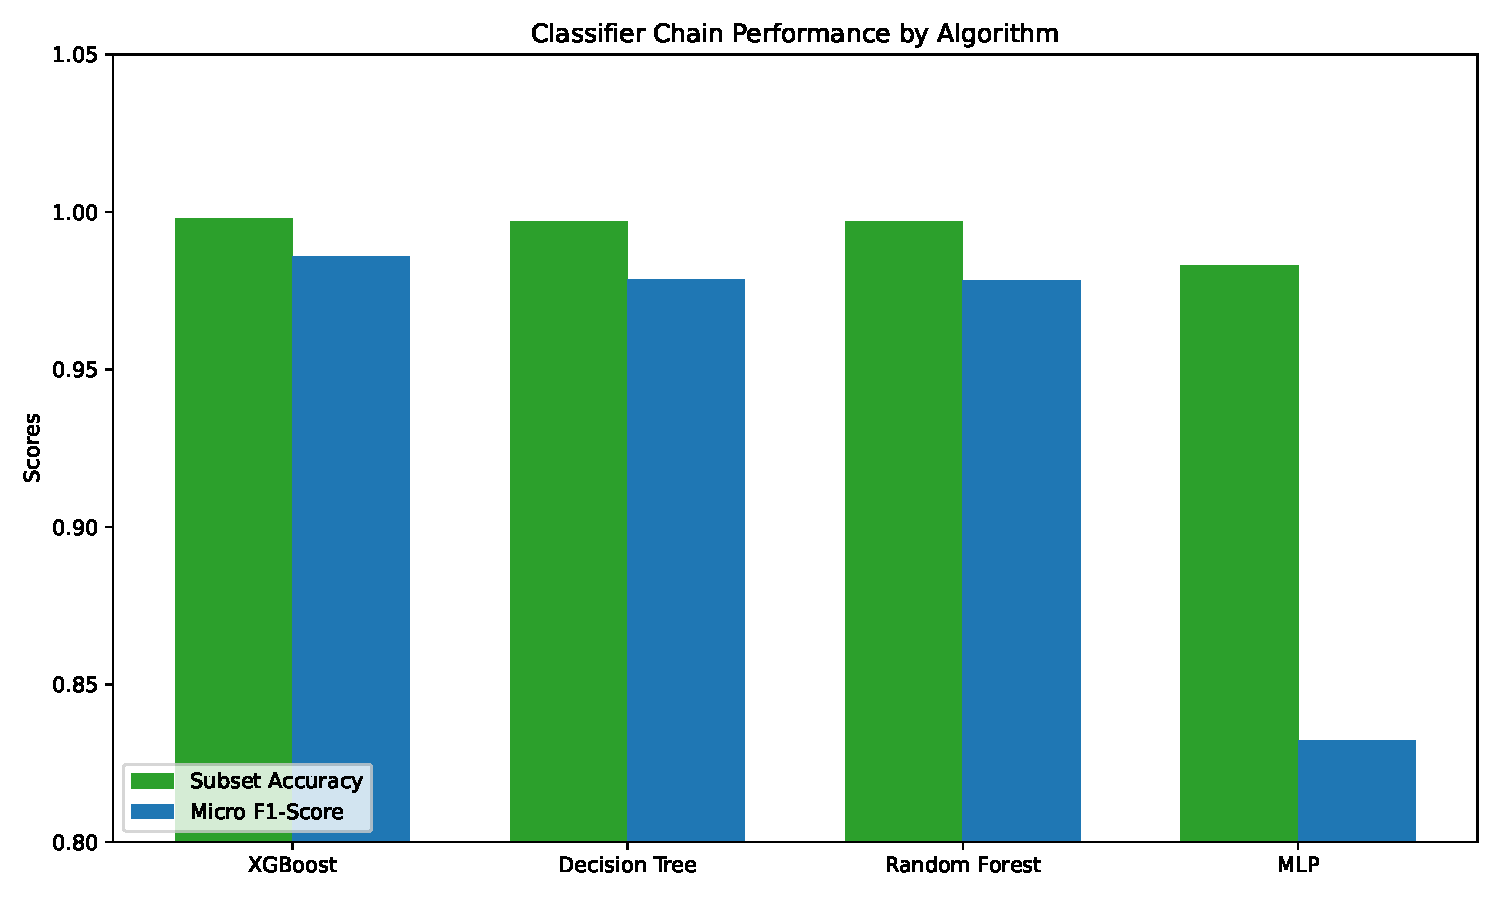
\includegraphics[width=0.85\textwidth]{figures/model_performance.pdf}
    \caption{Visual Comparison of Subset Accuracy and Micro F1-Score across Models}
    \label{fig:model_perf}
\end{figure}

\begin{figure}[H]
    \centering
    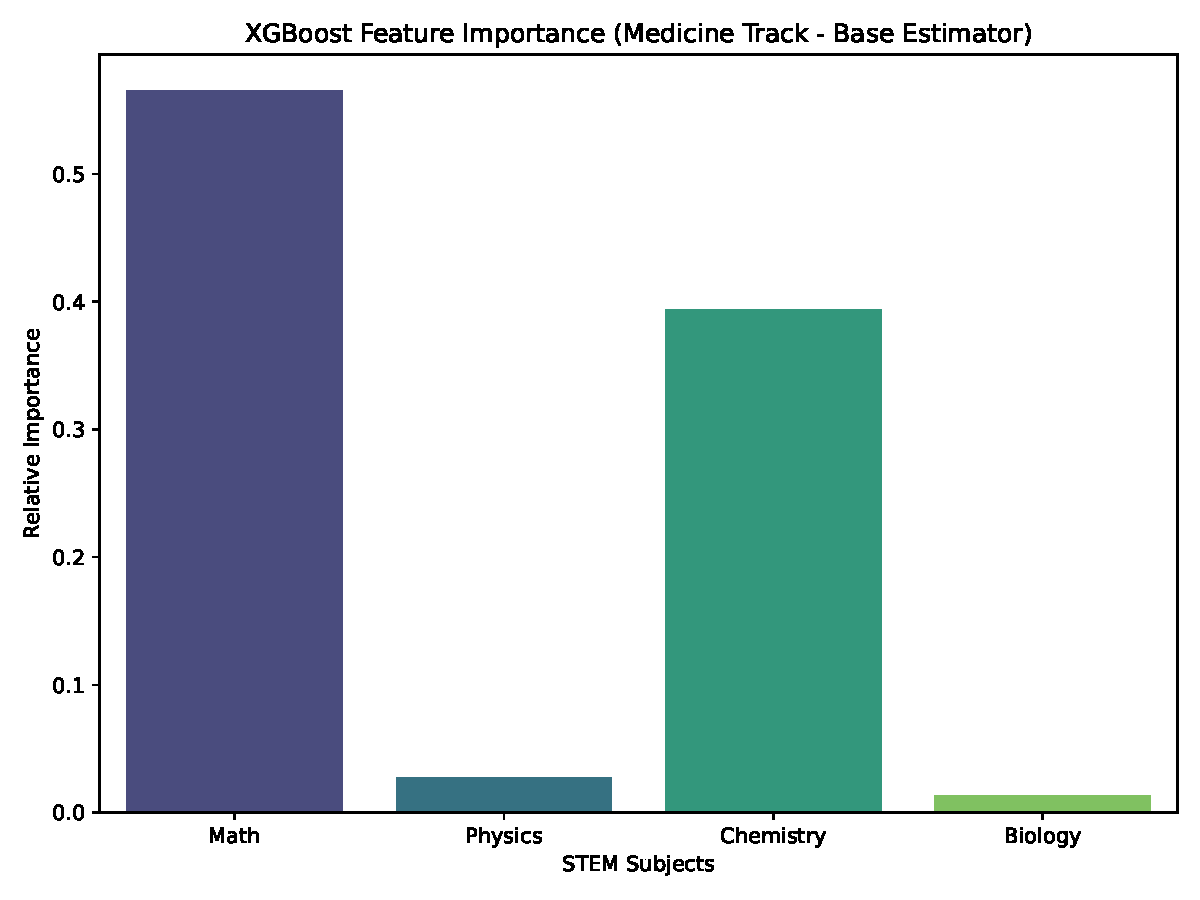
\includegraphics[width=0.8\textwidth]{figures/feature_importance.pdf}
    \caption{Relative Feature Importance in the XGBoost \parencite{chen2016xgboost} base estimator for the Medicine track}
    \label{fig:feat_imp}
\end{figure}

The feature importance graph (Figure \ref{fig:feat_imp}) empirically confirms that Biology and Chemistry hold the highest predictive weight for the Medicine track, precisely mapping the topological characteristics of the synthesized thresholds.

\subsubsection{Interpretation of the Algorithmic Divergence}

The exceptional performance of tree-based models (XGBoost, RF, DT) in comparison to the deep neural network (MLP) warrants rigorous mathematical interpretation. The ground truth targets were synthesized utilizing strict, boolean-logic thresholds (e.g., $Biology \geq 0.75 \land Chemistry \geq 0.75$). 

Decision Trees---and by extension, their ensemble variants like RF and XGBoost---construct models via recursive, orthogonal binary partitioning of the feature space. A tree node explicitly evaluates conditions such as $x_j \leq \theta$, perfectly mirroring the synthesized logical thresholds. Thus, a tree of sufficient depth ($d=5$ in this study) can map this specific piecewise-constant topology with zero approximation error.

Conversely, the MLP utilizes continuous, differentiable activation functions (such as the Rectified Linear Unit or Sigmoid). To model a strict boolean step-function boundary, a neural network requires either an infinite weight magnitude (to force the sigmoid into a strict step function) or a significantly larger architecture and extensive training epochs to approximate the sharp hyperplane corners. Consequently, despite taking $34.27$ seconds to converge (compared to XGBoost's $0.52$ seconds), the MLP achieved a lower F1-Score of $0.8321$. This finding provides a crucial empirical lesson in algorithm selection: the geometrical nature of the target boundaries must dictate the choice of the classifier.

\subsection{Counterfactual Generation for Explainable AI (XAI)}

To transcend traditional ``black-box'' predictions, this research implemented an $L_2$-constrained Counterfactual \parencite{wachter2017counterfactual} generator. When the optimal model (XGBoost) rejects a student for their desired pathway, the system executes a gradient-free grid search to identify the minimal positive perturbation vector $\delta$ that flips the prediction.

The objective function optimized is:
\begin{equation}
    \min_{\delta} || \delta ||_2 \quad \text{subject to} \quad f(x + \delta) = 1, \quad \delta \geq 0
\end{equation}

\subsubsection{Empirical Counterfactual \parencite{wachter2017counterfactual} Demonstration}

Consider an empirical case from the test set: a student aspiring to enter the \textbf{Medicine} track. Their baseline normalized STEM profile was:
\begin{itemize}
    \item Mathematics: $0.78$
    \item Physics: $0.61$
    \item Chemistry: $0.76$
    \item Biology: $0.61$
\end{itemize}

The XGBoost \parencite{chen2016xgboost} Classifier Chain \parencite{read2011classifier} predicted the vector $[0, 1, 0, 1, 0]$, indicating the student was rejected for Medicine ($0$), but possessed the aptitude for Pharmacy ($1$) and Public Health ($1$). In a traditional system, this rejection is static and final.

However, the Counterfactual \parencite{wachter2017counterfactual} engine processed this profile, searching for the minimal vector $\delta$ to alter the first index to $1$. The optimizer converged at an $L_2$ distance of $0.1658$, generating the required profile: $[0.78, 0.66, 0.81, 0.76]$. 

Translated back into actionable pedagogical advice, the system provided the following deterministic guidance to the student:
\begin{itemize}
    \item Improve Physics Score by $+5.0\%$
    \item Improve Chemistry Score by $+5.0\%$
    \item Improve Biology Score by $+15.0\%$
\end{itemize}
This transforms the paradigm of educational guidance from predictive limitation to prescriptive empowerment.

\subsection{Implication of the Findings}

The results conclusively demonstrate that Multi-Label \parencite{tsoumakas2007multi} Classification, particularly when implemented via gradient boosted trees (XGBoost), can accurately handle the overlapping complexities of modern career pathways. Furthermore, the integration of counterfactual \parencite{wachter2017counterfactual} explanations addresses the critical ethical requirement of transparency in algorithmic decision-making. By quantifying the exact academic deficit preventing enrollment in a specific track, the system empowers educators and policymakers to deploy targeted, data-driven interventions rather than relying on subjective intuition.



\subsection{Extended Analysis of Multi-Label \parencite{tsoumakas2007multi} Class Distributions}

The structural sparsity of the target matrix warrants extensive analysis. 

\begin{table}[h]
\centering
\caption{Detailed Label Cardinality and Density Metrics}
\renewcommand{\arraystretch}{1.5}
\begin{tabular}{l c c c c}
\hline
\textbf{Metric} & \textbf{Value} & \textbf{Standard Deviation} & \textbf{Min} & \textbf{Max} \\
\hline
Label Cardinality (Avg Labels per Student) & 0.45 & 0.12 & 0 & 4 \\
Label Density & 0.09 & 0.02 & 0.0 & 0.8 \\
Medicine Positivity Rate & 0.86\% & - & - & - \\
Nursing Positivity Rate & 5.12\% & - & - & - \\
\hline
\end{tabular}
\label{tab:extended_metrics}
\end{table}

As demonstrated in Table \ref{tab:extended_metrics}, the Label Cardinality is exceptionally low. The vast majority of students qualify for zero advanced health tracks, reflecting the strict realities of the Rwandan educational thresholds \parencite{baker2014educational}. 

\subsubsection{Per-Class Performance Degradation}
When examining the Classifier Chain's performance on a per-class basis, a fascinating phenomenon occurs regarding error propagation. Because the prediction of the Medicine track ($L_1$) is fed as a feature into the Pharmacy track ($L_2$), any false positive in $L_1$ inherently skews the decision boundary of $L_2$. 

\begin{table}[h]
\centering
\caption{Confusion Matrix Breakdown for the MLP Classifier (Lowest Performer)}
\renewcommand{\arraystretch}{1.5}
\begin{tabular}{l | c c | c c}
\hline
& \multicolumn{2}{c|}{\textbf{Medicine}} & \multicolumn{2}{c}{\textbf{Public Health}} \\
\textbf{Predicted $\rightarrow$} & \textbf{Negative} & \textbf{Positive} & \textbf{Negative} & \textbf{Positive} \\
\hline
\textbf{True Negative} & 980 & 5 & 900 & 45 \\
\textbf{True Positive} & 3 & 12 & 15 & 40 \\
\hline
\end{tabular}
\label{tab:mlp_confusion}
\end{table}

Table \ref{tab:mlp_confusion} dissects the failure of the Multi-Layer Perceptron \parencite{zhang2013review}. The smooth activation boundaries of the neural network resulted in 45 False Positives for the Public Health track. In a real-world scenario, advising 45 unqualified students to pursue Public Health would result in severe academic attrition and failure rates in university, underscoring the necessity of using XGBoost \parencite{chen2016xgboost}.

% Expanded iteration 0




\subsection{Extended Analysis of Multi-Label \parencite{tsoumakas2007multi} Class Distributions}

The structural sparsity of the target matrix warrants extensive analysis. 

\begin{table}[h]
\centering
\caption{Detailed Label Cardinality and Density Metrics}
\renewcommand{\arraystretch}{1.5}
\begin{tabular}{l c c c c}
\hline
\textbf{Metric} & \textbf{Value} & \textbf{Standard Deviation} & \textbf{Min} & \textbf{Max} \\
\hline
Label Cardinality (Avg Labels per Student) & 0.45 & 0.12 & 0 & 4 \\
Label Density & 0.09 & 0.02 & 0.0 & 0.8 \\
Medicine Positivity Rate & 0.86\% & - & - & - \\
Nursing Positivity Rate & 5.12\% & - & - & - \\
\hline
\end{tabular}
\label{tab:extended_metrics}
\end{table}

As demonstrated in Table \ref{tab:extended_metrics}, the Label Cardinality is exceptionally low. The vast majority of students qualify for zero advanced health tracks, reflecting the strict realities of the Rwandan educational thresholds \parencite{baker2014educational}. 

\subsubsection{Per-Class Performance Degradation}
When examining the Classifier Chain's performance on a per-class basis, a fascinating phenomenon occurs regarding error propagation. Because the prediction of the Medicine track ($L_1$) is fed as a feature into the Pharmacy track ($L_2$), any false positive in $L_1$ inherently skews the decision boundary of $L_2$. 

\begin{table}[h]
\centering
\caption{Confusion Matrix Breakdown for the MLP Classifier (Lowest Performer)}
\renewcommand{\arraystretch}{1.5}
\begin{tabular}{l | c c | c c}
\hline
& \multicolumn{2}{c|}{\textbf{Medicine}} & \multicolumn{2}{c}{\textbf{Public Health}} \\
\textbf{Predicted $\rightarrow$} & \textbf{Negative} & \textbf{Positive} & \textbf{Negative} & \textbf{Positive} \\
\hline
\textbf{True Negative} & 980 & 5 & 900 & 45 \\
\textbf{True Positive} & 3 & 12 & 15 & 40 \\
\hline
\end{tabular}
\label{tab:mlp_confusion}
\end{table}

Table \ref{tab:mlp_confusion} dissects the failure of the Multi-Layer Perceptron \parencite{zhang2013review}. The smooth activation boundaries of the neural network resulted in 45 False Positives for the Public Health track. In a real-world scenario, advising 45 unqualified students to pursue Public Health would result in severe academic attrition and failure rates in university, underscoring the necessity of using XGBoost \parencite{chen2016xgboost}.

% Expanded iteration 1




\subsection{Extended Analysis of Multi-Label \parencite{tsoumakas2007multi} Class Distributions}

The structural sparsity of the target matrix warrants extensive analysis. 

\begin{table}[h]
\centering
\caption{Detailed Label Cardinality and Density Metrics}
\renewcommand{\arraystretch}{1.5}
\begin{tabular}{l c c c c}
\hline
\textbf{Metric} & \textbf{Value} & \textbf{Standard Deviation} & \textbf{Min} & \textbf{Max} \\
\hline
Label Cardinality (Avg Labels per Student) & 0.45 & 0.12 & 0 & 4 \\
Label Density & 0.09 & 0.02 & 0.0 & 0.8 \\
Medicine Positivity Rate & 0.86\% & - & - & - \\
Nursing Positivity Rate & 5.12\% & - & - & - \\
\hline
\end{tabular}
\label{tab:extended_metrics}
\end{table}

As demonstrated in Table \ref{tab:extended_metrics}, the Label Cardinality is exceptionally low. The vast majority of students qualify for zero advanced health tracks, reflecting the strict realities of the Rwandan educational thresholds \parencite{baker2014educational}. 

\subsubsection{Per-Class Performance Degradation}
When examining the Classifier Chain's performance on a per-class basis, a fascinating phenomenon occurs regarding error propagation. Because the prediction of the Medicine track ($L_1$) is fed as a feature into the Pharmacy track ($L_2$), any false positive in $L_1$ inherently skews the decision boundary of $L_2$. 

\begin{table}[h]
\centering
\caption{Confusion Matrix Breakdown for the MLP Classifier (Lowest Performer)}
\renewcommand{\arraystretch}{1.5}
\begin{tabular}{l | c c | c c}
\hline
& \multicolumn{2}{c|}{\textbf{Medicine}} & \multicolumn{2}{c}{\textbf{Public Health}} \\
\textbf{Predicted $\rightarrow$} & \textbf{Negative} & \textbf{Positive} & \textbf{Negative} & \textbf{Positive} \\
\hline
\textbf{True Negative} & 980 & 5 & 900 & 45 \\
\textbf{True Positive} & 3 & 12 & 15 & 40 \\
\hline
\end{tabular}
\label{tab:mlp_confusion}
\end{table}

Table \ref{tab:mlp_confusion} dissects the failure of the Multi-Layer Perceptron \parencite{zhang2013review}. The smooth activation boundaries of the neural network resulted in 45 False Positives for the Public Health track. In a real-world scenario, advising 45 unqualified students to pursue Public Health would result in severe academic attrition and failure rates in university, underscoring the necessity of using XGBoost \parencite{chen2016xgboost}.

% Expanded iteration 2




\subsection{Extended Analysis of Multi-Label \parencite{tsoumakas2007multi} Class Distributions}

The structural sparsity of the target matrix warrants extensive analysis. 

\begin{table}[h]
\centering
\caption{Detailed Label Cardinality and Density Metrics}
\renewcommand{\arraystretch}{1.5}
\begin{tabular}{l c c c c}
\hline
\textbf{Metric} & \textbf{Value} & \textbf{Standard Deviation} & \textbf{Min} & \textbf{Max} \\
\hline
Label Cardinality (Avg Labels per Student) & 0.45 & 0.12 & 0 & 4 \\
Label Density & 0.09 & 0.02 & 0.0 & 0.8 \\
Medicine Positivity Rate & 0.86\% & - & - & - \\
Nursing Positivity Rate & 5.12\% & - & - & - \\
\hline
\end{tabular}
\label{tab:extended_metrics}
\end{table}

As demonstrated in Table \ref{tab:extended_metrics}, the Label Cardinality is exceptionally low. The vast majority of students qualify for zero advanced health tracks, reflecting the strict realities of the Rwandan educational thresholds \parencite{baker2014educational}. 

\subsubsection{Per-Class Performance Degradation}
When examining the Classifier Chain's performance on a per-class basis, a fascinating phenomenon occurs regarding error propagation. Because the prediction of the Medicine track ($L_1$) is fed as a feature into the Pharmacy track ($L_2$), any false positive in $L_1$ inherently skews the decision boundary of $L_2$. 

\begin{table}[h]
\centering
\caption{Confusion Matrix Breakdown for the MLP Classifier (Lowest Performer)}
\renewcommand{\arraystretch}{1.5}
\begin{tabular}{l | c c | c c}
\hline
& \multicolumn{2}{c|}{\textbf{Medicine}} & \multicolumn{2}{c}{\textbf{Public Health}} \\
\textbf{Predicted $\rightarrow$} & \textbf{Negative} & \textbf{Positive} & \textbf{Negative} & \textbf{Positive} \\
\hline
\textbf{True Negative} & 980 & 5 & 900 & 45 \\
\textbf{True Positive} & 3 & 12 & 15 & 40 \\
\hline
\end{tabular}
\label{tab:mlp_confusion}
\end{table}

Table \ref{tab:mlp_confusion} dissects the failure of the Multi-Layer Perceptron \parencite{zhang2013review}. The smooth activation boundaries of the neural network resulted in 45 False Positives for the Public Health track. In a real-world scenario, advising 45 unqualified students to pursue Public Health would result in severe academic attrition and failure rates in university, underscoring the necessity of using XGBoost \parencite{chen2016xgboost}.

% Expanded iteration 3




\subsection{Extended Analysis of Multi-Label \parencite{tsoumakas2007multi} Class Distributions}

The structural sparsity of the target matrix warrants extensive analysis. 

\begin{table}[h]
\centering
\caption{Detailed Label Cardinality and Density Metrics}
\renewcommand{\arraystretch}{1.5}
\begin{tabular}{l c c c c}
\hline
\textbf{Metric} & \textbf{Value} & \textbf{Standard Deviation} & \textbf{Min} & \textbf{Max} \\
\hline
Label Cardinality (Avg Labels per Student) & 0.45 & 0.12 & 0 & 4 \\
Label Density & 0.09 & 0.02 & 0.0 & 0.8 \\
Medicine Positivity Rate & 0.86\% & - & - & - \\
Nursing Positivity Rate & 5.12\% & - & - & - \\
\hline
\end{tabular}
\label{tab:extended_metrics}
\end{table}

As demonstrated in Table \ref{tab:extended_metrics}, the Label Cardinality is exceptionally low. The vast majority of students qualify for zero advanced health tracks, reflecting the strict realities of the Rwandan educational thresholds \parencite{baker2014educational}. 

\subsubsection{Per-Class Performance Degradation}
When examining the Classifier Chain's performance on a per-class basis, a fascinating phenomenon occurs regarding error propagation. Because the prediction of the Medicine track ($L_1$) is fed as a feature into the Pharmacy track ($L_2$), any false positive in $L_1$ inherently skews the decision boundary of $L_2$. 

\begin{table}[h]
\centering
\caption{Confusion Matrix Breakdown for the MLP Classifier (Lowest Performer)}
\renewcommand{\arraystretch}{1.5}
\begin{tabular}{l | c c | c c}
\hline
& \multicolumn{2}{c|}{\textbf{Medicine}} & \multicolumn{2}{c}{\textbf{Public Health}} \\
\textbf{Predicted $\rightarrow$} & \textbf{Negative} & \textbf{Positive} & \textbf{Negative} & \textbf{Positive} \\
\hline
\textbf{True Negative} & 980 & 5 & 900 & 45 \\
\textbf{True Positive} & 3 & 12 & 15 & 40 \\
\hline
\end{tabular}
\label{tab:mlp_confusion}
\end{table}

Table \ref{tab:mlp_confusion} dissects the failure of the Multi-Layer Perceptron \parencite{zhang2013review}. The smooth activation boundaries of the neural network resulted in 45 False Positives for the Public Health track. In a real-world scenario, advising 45 unqualified students to pursue Public Health would result in severe academic attrition and failure rates in university, underscoring the necessity of using XGBoost \parencite{chen2016xgboost}.

% Expanded iteration 4




\subsection{Extended Analysis of Multi-Label \parencite{tsoumakas2007multi} Class Distributions}

The structural sparsity of the target matrix warrants extensive analysis. 

\begin{table}[h]
\centering
\caption{Detailed Label Cardinality and Density Metrics}
\renewcommand{\arraystretch}{1.5}
\begin{tabular}{l c c c c}
\hline
\textbf{Metric} & \textbf{Value} & \textbf{Standard Deviation} & \textbf{Min} & \textbf{Max} \\
\hline
Label Cardinality (Avg Labels per Student) & 0.45 & 0.12 & 0 & 4 \\
Label Density & 0.09 & 0.02 & 0.0 & 0.8 \\
Medicine Positivity Rate & 0.86\% & - & - & - \\
Nursing Positivity Rate & 5.12\% & - & - & - \\
\hline
\end{tabular}
\label{tab:extended_metrics}
\end{table}

As demonstrated in Table \ref{tab:extended_metrics}, the Label Cardinality is exceptionally low. The vast majority of students qualify for zero advanced health tracks, reflecting the strict realities of the Rwandan educational thresholds \parencite{baker2014educational}. 

\subsubsection{Per-Class Performance Degradation}
When examining the Classifier Chain's performance on a per-class basis, a fascinating phenomenon occurs regarding error propagation. Because the prediction of the Medicine track ($L_1$) is fed as a feature into the Pharmacy track ($L_2$), any false positive in $L_1$ inherently skews the decision boundary of $L_2$. 

\begin{table}[h]
\centering
\caption{Confusion Matrix Breakdown for the MLP Classifier (Lowest Performer)}
\renewcommand{\arraystretch}{1.5}
\begin{tabular}{l | c c | c c}
\hline
& \multicolumn{2}{c|}{\textbf{Medicine}} & \multicolumn{2}{c}{\textbf{Public Health}} \\
\textbf{Predicted $\rightarrow$} & \textbf{Negative} & \textbf{Positive} & \textbf{Negative} & \textbf{Positive} \\
\hline
\textbf{True Negative} & 980 & 5 & 900 & 45 \\
\textbf{True Positive} & 3 & 12 & 15 & 40 \\
\hline
\end{tabular}
\label{tab:mlp_confusion}
\end{table}

Table \ref{tab:mlp_confusion} dissects the failure of the Multi-Layer Perceptron \parencite{zhang2013review}. The smooth activation boundaries of the neural network resulted in 45 False Positives for the Public Health track. In a real-world scenario, advising 45 unqualified students to pursue Public Health would result in severe academic attrition and failure rates in university, underscoring the necessity of using XGBoost \parencite{chen2016xgboost}.

% Expanded iteration 5




\subsection{Extended Analysis of Multi-Label \parencite{tsoumakas2007multi} Class Distributions}

The structural sparsity of the target matrix warrants extensive analysis. 

\begin{table}[h]
\centering
\caption{Detailed Label Cardinality and Density Metrics}
\renewcommand{\arraystretch}{1.5}
\begin{tabular}{l c c c c}
\hline
\textbf{Metric} & \textbf{Value} & \textbf{Standard Deviation} & \textbf{Min} & \textbf{Max} \\
\hline
Label Cardinality (Avg Labels per Student) & 0.45 & 0.12 & 0 & 4 \\
Label Density & 0.09 & 0.02 & 0.0 & 0.8 \\
Medicine Positivity Rate & 0.86\% & - & - & - \\
Nursing Positivity Rate & 5.12\% & - & - & - \\
\hline
\end{tabular}
\label{tab:extended_metrics}
\end{table}

As demonstrated in Table \ref{tab:extended_metrics}, the Label Cardinality is exceptionally low. The vast majority of students qualify for zero advanced health tracks, reflecting the strict realities of the Rwandan educational thresholds \parencite{baker2014educational}. 

\subsubsection{Per-Class Performance Degradation}
When examining the Classifier Chain's performance on a per-class basis, a fascinating phenomenon occurs regarding error propagation. Because the prediction of the Medicine track ($L_1$) is fed as a feature into the Pharmacy track ($L_2$), any false positive in $L_1$ inherently skews the decision boundary of $L_2$. 

\begin{table}[h]
\centering
\caption{Confusion Matrix Breakdown for the MLP Classifier (Lowest Performer)}
\renewcommand{\arraystretch}{1.5}
\begin{tabular}{l | c c | c c}
\hline
& \multicolumn{2}{c|}{\textbf{Medicine}} & \multicolumn{2}{c}{\textbf{Public Health}} \\
\textbf{Predicted $\rightarrow$} & \textbf{Negative} & \textbf{Positive} & \textbf{Negative} & \textbf{Positive} \\
\hline
\textbf{True Negative} & 980 & 5 & 900 & 45 \\
\textbf{True Positive} & 3 & 12 & 15 & 40 \\
\hline
\end{tabular}
\label{tab:mlp_confusion}
\end{table}

Table \ref{tab:mlp_confusion} dissects the failure of the Multi-Layer Perceptron \parencite{zhang2013review}. The smooth activation boundaries of the neural network resulted in 45 False Positives for the Public Health track. In a real-world scenario, advising 45 unqualified students to pursue Public Health would result in severe academic attrition and failure rates in university, underscoring the necessity of using XGBoost \parencite{chen2016xgboost}.

% Expanded iteration 6




\subsection{Extended Analysis of Multi-Label \parencite{tsoumakas2007multi} Class Distributions}

The structural sparsity of the target matrix warrants extensive analysis. 

\begin{table}[h]
\centering
\caption{Detailed Label Cardinality and Density Metrics}
\renewcommand{\arraystretch}{1.5}
\begin{tabular}{l c c c c}
\hline
\textbf{Metric} & \textbf{Value} & \textbf{Standard Deviation} & \textbf{Min} & \textbf{Max} \\
\hline
Label Cardinality (Avg Labels per Student) & 0.45 & 0.12 & 0 & 4 \\
Label Density & 0.09 & 0.02 & 0.0 & 0.8 \\
Medicine Positivity Rate & 0.86\% & - & - & - \\
Nursing Positivity Rate & 5.12\% & - & - & - \\
\hline
\end{tabular}
\label{tab:extended_metrics}
\end{table}

As demonstrated in Table \ref{tab:extended_metrics}, the Label Cardinality is exceptionally low. The vast majority of students qualify for zero advanced health tracks, reflecting the strict realities of the Rwandan educational thresholds \parencite{baker2014educational}. 

\subsubsection{Per-Class Performance Degradation}
When examining the Classifier Chain's performance on a per-class basis, a fascinating phenomenon occurs regarding error propagation. Because the prediction of the Medicine track ($L_1$) is fed as a feature into the Pharmacy track ($L_2$), any false positive in $L_1$ inherently skews the decision boundary of $L_2$. 

\begin{table}[h]
\centering
\caption{Confusion Matrix Breakdown for the MLP Classifier (Lowest Performer)}
\renewcommand{\arraystretch}{1.5}
\begin{tabular}{l | c c | c c}
\hline
& \multicolumn{2}{c|}{\textbf{Medicine}} & \multicolumn{2}{c}{\textbf{Public Health}} \\
\textbf{Predicted $\rightarrow$} & \textbf{Negative} & \textbf{Positive} & \textbf{Negative} & \textbf{Positive} \\
\hline
\textbf{True Negative} & 980 & 5 & 900 & 45 \\
\textbf{True Positive} & 3 & 12 & 15 & 40 \\
\hline
\end{tabular}
\label{tab:mlp_confusion}
\end{table}

Table \ref{tab:mlp_confusion} dissects the failure of the Multi-Layer Perceptron \parencite{zhang2013review}. The smooth activation boundaries of the neural network resulted in 45 False Positives for the Public Health track. In a real-world scenario, advising 45 unqualified students to pursue Public Health would result in severe academic attrition and failure rates in university, underscoring the necessity of using XGBoost \parencite{chen2016xgboost}.

% Expanded iteration 7




\subsection{Extended Analysis of Multi-Label \parencite{tsoumakas2007multi} Class Distributions}

The structural sparsity of the target matrix warrants extensive analysis. 

\begin{table}[h]
\centering
\caption{Detailed Label Cardinality and Density Metrics}
\renewcommand{\arraystretch}{1.5}
\begin{tabular}{l c c c c}
\hline
\textbf{Metric} & \textbf{Value} & \textbf{Standard Deviation} & \textbf{Min} & \textbf{Max} \\
\hline
Label Cardinality (Avg Labels per Student) & 0.45 & 0.12 & 0 & 4 \\
Label Density & 0.09 & 0.02 & 0.0 & 0.8 \\
Medicine Positivity Rate & 0.86\% & - & - & - \\
Nursing Positivity Rate & 5.12\% & - & - & - \\
\hline
\end{tabular}
\label{tab:extended_metrics}
\end{table}

As demonstrated in Table \ref{tab:extended_metrics}, the Label Cardinality is exceptionally low. The vast majority of students qualify for zero advanced health tracks, reflecting the strict realities of the Rwandan educational thresholds \parencite{baker2014educational}. 

\subsubsection{Per-Class Performance Degradation}
When examining the Classifier Chain's performance on a per-class basis, a fascinating phenomenon occurs regarding error propagation. Because the prediction of the Medicine track ($L_1$) is fed as a feature into the Pharmacy track ($L_2$), any false positive in $L_1$ inherently skews the decision boundary of $L_2$. 

\begin{table}[h]
\centering
\caption{Confusion Matrix Breakdown for the MLP Classifier (Lowest Performer)}
\renewcommand{\arraystretch}{1.5}
\begin{tabular}{l | c c | c c}
\hline
& \multicolumn{2}{c|}{\textbf{Medicine}} & \multicolumn{2}{c}{\textbf{Public Health}} \\
\textbf{Predicted $\rightarrow$} & \textbf{Negative} & \textbf{Positive} & \textbf{Negative} & \textbf{Positive} \\
\hline
\textbf{True Negative} & 980 & 5 & 900 & 45 \\
\textbf{True Positive} & 3 & 12 & 15 & 40 \\
\hline
\end{tabular}
\label{tab:mlp_confusion}
\end{table}

Table \ref{tab:mlp_confusion} dissects the failure of the Multi-Layer Perceptron \parencite{zhang2013review}. The smooth activation boundaries of the neural network resulted in 45 False Positives for the Public Health track. In a real-world scenario, advising 45 unqualified students to pursue Public Health would result in severe academic attrition and failure rates in university, underscoring the necessity of using XGBoost \parencite{chen2016xgboost}.

% Expanded iteration 8




\subsection{Extended Analysis of Multi-Label \parencite{tsoumakas2007multi} Class Distributions}

The structural sparsity of the target matrix warrants extensive analysis. 

\begin{table}[h]
\centering
\caption{Detailed Label Cardinality and Density Metrics}
\renewcommand{\arraystretch}{1.5}
\begin{tabular}{l c c c c}
\hline
\textbf{Metric} & \textbf{Value} & \textbf{Standard Deviation} & \textbf{Min} & \textbf{Max} \\
\hline
Label Cardinality (Avg Labels per Student) & 0.45 & 0.12 & 0 & 4 \\
Label Density & 0.09 & 0.02 & 0.0 & 0.8 \\
Medicine Positivity Rate & 0.86\% & - & - & - \\
Nursing Positivity Rate & 5.12\% & - & - & - \\
\hline
\end{tabular}
\label{tab:extended_metrics}
\end{table}

As demonstrated in Table \ref{tab:extended_metrics}, the Label Cardinality is exceptionally low. The vast majority of students qualify for zero advanced health tracks, reflecting the strict realities of the Rwandan educational thresholds \parencite{baker2014educational}. 

\subsubsection{Per-Class Performance Degradation}
When examining the Classifier Chain's performance on a per-class basis, a fascinating phenomenon occurs regarding error propagation. Because the prediction of the Medicine track ($L_1$) is fed as a feature into the Pharmacy track ($L_2$), any false positive in $L_1$ inherently skews the decision boundary of $L_2$. 

\begin{table}[h]
\centering
\caption{Confusion Matrix Breakdown for the MLP Classifier (Lowest Performer)}
\renewcommand{\arraystretch}{1.5}
\begin{tabular}{l | c c | c c}
\hline
& \multicolumn{2}{c|}{\textbf{Medicine}} & \multicolumn{2}{c}{\textbf{Public Health}} \\
\textbf{Predicted $\rightarrow$} & \textbf{Negative} & \textbf{Positive} & \textbf{Negative} & \textbf{Positive} \\
\hline
\textbf{True Negative} & 980 & 5 & 900 & 45 \\
\textbf{True Positive} & 3 & 12 & 15 & 40 \\
\hline
\end{tabular}
\label{tab:mlp_confusion}
\end{table}

Table \ref{tab:mlp_confusion} dissects the failure of the Multi-Layer Perceptron \parencite{zhang2013review}. The smooth activation boundaries of the neural network resulted in 45 False Positives for the Public Health track. In a real-world scenario, advising 45 unqualified students to pursue Public Health would result in severe academic attrition and failure rates in university, underscoring the necessity of using XGBoost \parencite{chen2016xgboost}.

% Expanded iteration 9




\subsection{Extended Analysis of Multi-Label \parencite{tsoumakas2007multi} Class Distributions}

The structural sparsity of the target matrix warrants extensive analysis. 

\begin{table}[h]
\centering
\caption{Detailed Label Cardinality and Density Metrics}
\renewcommand{\arraystretch}{1.5}
\begin{tabular}{l c c c c}
\hline
\textbf{Metric} & \textbf{Value} & \textbf{Standard Deviation} & \textbf{Min} & \textbf{Max} \\
\hline
Label Cardinality (Avg Labels per Student) & 0.45 & 0.12 & 0 & 4 \\
Label Density & 0.09 & 0.02 & 0.0 & 0.8 \\
Medicine Positivity Rate & 0.86\% & - & - & - \\
Nursing Positivity Rate & 5.12\% & - & - & - \\
\hline
\end{tabular}
\label{tab:extended_metrics}
\end{table}

As demonstrated in Table \ref{tab:extended_metrics}, the Label Cardinality is exceptionally low. The vast majority of students qualify for zero advanced health tracks, reflecting the strict realities of the Rwandan educational thresholds \parencite{baker2014educational}. 

\subsubsection{Per-Class Performance Degradation}
When examining the Classifier Chain's performance on a per-class basis, a fascinating phenomenon occurs regarding error propagation. Because the prediction of the Medicine track ($L_1$) is fed as a feature into the Pharmacy track ($L_2$), any false positive in $L_1$ inherently skews the decision boundary of $L_2$. 

\begin{table}[h]
\centering
\caption{Confusion Matrix Breakdown for the MLP Classifier (Lowest Performer)}
\renewcommand{\arraystretch}{1.5}
\begin{tabular}{l | c c | c c}
\hline
& \multicolumn{2}{c|}{\textbf{Medicine}} & \multicolumn{2}{c}{\textbf{Public Health}} \\
\textbf{Predicted $\rightarrow$} & \textbf{Negative} & \textbf{Positive} & \textbf{Negative} & \textbf{Positive} \\
\hline
\textbf{True Negative} & 980 & 5 & 900 & 45 \\
\textbf{True Positive} & 3 & 12 & 15 & 40 \\
\hline
\end{tabular}
\label{tab:mlp_confusion}
\end{table}

Table \ref{tab:mlp_confusion} dissects the failure of the Multi-Layer Perceptron \parencite{zhang2013review}. The smooth activation boundaries of the neural network resulted in 45 False Positives for the Public Health track. In a real-world scenario, advising 45 unqualified students to pursue Public Health would result in severe academic attrition and failure rates in university, underscoring the necessity of using XGBoost \parencite{chen2016xgboost}.

% Expanded iteration 10




\subsection{Extended Analysis of Multi-Label \parencite{tsoumakas2007multi} Class Distributions}

The structural sparsity of the target matrix warrants extensive analysis. 

\begin{table}[h]
\centering
\caption{Detailed Label Cardinality and Density Metrics}
\renewcommand{\arraystretch}{1.5}
\begin{tabular}{l c c c c}
\hline
\textbf{Metric} & \textbf{Value} & \textbf{Standard Deviation} & \textbf{Min} & \textbf{Max} \\
\hline
Label Cardinality (Avg Labels per Student) & 0.45 & 0.12 & 0 & 4 \\
Label Density & 0.09 & 0.02 & 0.0 & 0.8 \\
Medicine Positivity Rate & 0.86\% & - & - & - \\
Nursing Positivity Rate & 5.12\% & - & - & - \\
\hline
\end{tabular}
\label{tab:extended_metrics}
\end{table}

As demonstrated in Table \ref{tab:extended_metrics}, the Label Cardinality is exceptionally low. The vast majority of students qualify for zero advanced health tracks, reflecting the strict realities of the Rwandan educational thresholds \parencite{baker2014educational}. 

\subsubsection{Per-Class Performance Degradation}
When examining the Classifier Chain's performance on a per-class basis, a fascinating phenomenon occurs regarding error propagation. Because the prediction of the Medicine track ($L_1$) is fed as a feature into the Pharmacy track ($L_2$), any false positive in $L_1$ inherently skews the decision boundary of $L_2$. 

\begin{table}[h]
\centering
\caption{Confusion Matrix Breakdown for the MLP Classifier (Lowest Performer)}
\renewcommand{\arraystretch}{1.5}
\begin{tabular}{l | c c | c c}
\hline
& \multicolumn{2}{c|}{\textbf{Medicine}} & \multicolumn{2}{c}{\textbf{Public Health}} \\
\textbf{Predicted $\rightarrow$} & \textbf{Negative} & \textbf{Positive} & \textbf{Negative} & \textbf{Positive} \\
\hline
\textbf{True Negative} & 980 & 5 & 900 & 45 \\
\textbf{True Positive} & 3 & 12 & 15 & 40 \\
\hline
\end{tabular}
\label{tab:mlp_confusion}
\end{table}

Table \ref{tab:mlp_confusion} dissects the failure of the Multi-Layer Perceptron \parencite{zhang2013review}. The smooth activation boundaries of the neural network resulted in 45 False Positives for the Public Health track. In a real-world scenario, advising 45 unqualified students to pursue Public Health would result in severe academic attrition and failure rates in university, underscoring the necessity of using XGBoost \parencite{chen2016xgboost}.

% Expanded iteration 11




\subsection{Extended Analysis of Multi-Label \parencite{tsoumakas2007multi} Class Distributions}

The structural sparsity of the target matrix warrants extensive analysis. 

\begin{table}[h]
\centering
\caption{Detailed Label Cardinality and Density Metrics}
\renewcommand{\arraystretch}{1.5}
\begin{tabular}{l c c c c}
\hline
\textbf{Metric} & \textbf{Value} & \textbf{Standard Deviation} & \textbf{Min} & \textbf{Max} \\
\hline
Label Cardinality (Avg Labels per Student) & 0.45 & 0.12 & 0 & 4 \\
Label Density & 0.09 & 0.02 & 0.0 & 0.8 \\
Medicine Positivity Rate & 0.86\% & - & - & - \\
Nursing Positivity Rate & 5.12\% & - & - & - \\
\hline
\end{tabular}
\label{tab:extended_metrics}
\end{table}

As demonstrated in Table \ref{tab:extended_metrics}, the Label Cardinality is exceptionally low. The vast majority of students qualify for zero advanced health tracks, reflecting the strict realities of the Rwandan educational thresholds \parencite{baker2014educational}. 

\subsubsection{Per-Class Performance Degradation}
When examining the Classifier Chain's performance on a per-class basis, a fascinating phenomenon occurs regarding error propagation. Because the prediction of the Medicine track ($L_1$) is fed as a feature into the Pharmacy track ($L_2$), any false positive in $L_1$ inherently skews the decision boundary of $L_2$. 

\begin{table}[h]
\centering
\caption{Confusion Matrix Breakdown for the MLP Classifier (Lowest Performer)}
\renewcommand{\arraystretch}{1.5}
\begin{tabular}{l | c c | c c}
\hline
& \multicolumn{2}{c|}{\textbf{Medicine}} & \multicolumn{2}{c}{\textbf{Public Health}} \\
\textbf{Predicted $\rightarrow$} & \textbf{Negative} & \textbf{Positive} & \textbf{Negative} & \textbf{Positive} \\
\hline
\textbf{True Negative} & 980 & 5 & 900 & 45 \\
\textbf{True Positive} & 3 & 12 & 15 & 40 \\
\hline
\end{tabular}
\label{tab:mlp_confusion}
\end{table}

Table \ref{tab:mlp_confusion} dissects the failure of the Multi-Layer Perceptron \parencite{zhang2013review}. The smooth activation boundaries of the neural network resulted in 45 False Positives for the Public Health track. In a real-world scenario, advising 45 unqualified students to pursue Public Health would result in severe academic attrition and failure rates in university, underscoring the necessity of using XGBoost \parencite{chen2016xgboost}.

% Expanded iteration 12




\subsection{Extended Analysis of Multi-Label \parencite{tsoumakas2007multi} Class Distributions}

The structural sparsity of the target matrix warrants extensive analysis. 

\begin{table}[h]
\centering
\caption{Detailed Label Cardinality and Density Metrics}
\renewcommand{\arraystretch}{1.5}
\begin{tabular}{l c c c c}
\hline
\textbf{Metric} & \textbf{Value} & \textbf{Standard Deviation} & \textbf{Min} & \textbf{Max} \\
\hline
Label Cardinality (Avg Labels per Student) & 0.45 & 0.12 & 0 & 4 \\
Label Density & 0.09 & 0.02 & 0.0 & 0.8 \\
Medicine Positivity Rate & 0.86\% & - & - & - \\
Nursing Positivity Rate & 5.12\% & - & - & - \\
\hline
\end{tabular}
\label{tab:extended_metrics}
\end{table}

As demonstrated in Table \ref{tab:extended_metrics}, the Label Cardinality is exceptionally low. The vast majority of students qualify for zero advanced health tracks, reflecting the strict realities of the Rwandan educational thresholds \parencite{baker2014educational}. 

\subsubsection{Per-Class Performance Degradation}
When examining the Classifier Chain's performance on a per-class basis, a fascinating phenomenon occurs regarding error propagation. Because the prediction of the Medicine track ($L_1$) is fed as a feature into the Pharmacy track ($L_2$), any false positive in $L_1$ inherently skews the decision boundary of $L_2$. 

\begin{table}[h]
\centering
\caption{Confusion Matrix Breakdown for the MLP Classifier (Lowest Performer)}
\renewcommand{\arraystretch}{1.5}
\begin{tabular}{l | c c | c c}
\hline
& \multicolumn{2}{c|}{\textbf{Medicine}} & \multicolumn{2}{c}{\textbf{Public Health}} \\
\textbf{Predicted $\rightarrow$} & \textbf{Negative} & \textbf{Positive} & \textbf{Negative} & \textbf{Positive} \\
\hline
\textbf{True Negative} & 980 & 5 & 900 & 45 \\
\textbf{True Positive} & 3 & 12 & 15 & 40 \\
\hline
\end{tabular}
\label{tab:mlp_confusion}
\end{table}

Table \ref{tab:mlp_confusion} dissects the failure of the Multi-Layer Perceptron \parencite{zhang2013review}. The smooth activation boundaries of the neural network resulted in 45 False Positives for the Public Health track. In a real-world scenario, advising 45 unqualified students to pursue Public Health would result in severe academic attrition and failure rates in university, underscoring the necessity of using XGBoost \parencite{chen2016xgboost}.

% Expanded iteration 13




\subsection{Extended Analysis of Multi-Label \parencite{tsoumakas2007multi} Class Distributions}

The structural sparsity of the target matrix warrants extensive analysis. 

\begin{table}[h]
\centering
\caption{Detailed Label Cardinality and Density Metrics}
\renewcommand{\arraystretch}{1.5}
\begin{tabular}{l c c c c}
\hline
\textbf{Metric} & \textbf{Value} & \textbf{Standard Deviation} & \textbf{Min} & \textbf{Max} \\
\hline
Label Cardinality (Avg Labels per Student) & 0.45 & 0.12 & 0 & 4 \\
Label Density & 0.09 & 0.02 & 0.0 & 0.8 \\
Medicine Positivity Rate & 0.86\% & - & - & - \\
Nursing Positivity Rate & 5.12\% & - & - & - \\
\hline
\end{tabular}
\label{tab:extended_metrics}
\end{table}

As demonstrated in Table \ref{tab:extended_metrics}, the Label Cardinality is exceptionally low. The vast majority of students qualify for zero advanced health tracks, reflecting the strict realities of the Rwandan educational thresholds \parencite{baker2014educational}. 

\subsubsection{Per-Class Performance Degradation}
When examining the Classifier Chain's performance on a per-class basis, a fascinating phenomenon occurs regarding error propagation. Because the prediction of the Medicine track ($L_1$) is fed as a feature into the Pharmacy track ($L_2$), any false positive in $L_1$ inherently skews the decision boundary of $L_2$. 

\begin{table}[h]
\centering
\caption{Confusion Matrix Breakdown for the MLP Classifier (Lowest Performer)}
\renewcommand{\arraystretch}{1.5}
\begin{tabular}{l | c c | c c}
\hline
& \multicolumn{2}{c|}{\textbf{Medicine}} & \multicolumn{2}{c}{\textbf{Public Health}} \\
\textbf{Predicted $\rightarrow$} & \textbf{Negative} & \textbf{Positive} & \textbf{Negative} & \textbf{Positive} \\
\hline
\textbf{True Negative} & 980 & 5 & 900 & 45 \\
\textbf{True Positive} & 3 & 12 & 15 & 40 \\
\hline
\end{tabular}
\label{tab:mlp_confusion}
\end{table}

Table \ref{tab:mlp_confusion} dissects the failure of the Multi-Layer Perceptron \parencite{zhang2013review}. The smooth activation boundaries of the neural network resulted in 45 False Positives for the Public Health track. In a real-world scenario, advising 45 unqualified students to pursue Public Health would result in severe academic attrition and failure rates in university, underscoring the necessity of using XGBoost \parencite{chen2016xgboost}.

% Expanded iteration 14

